\documentclass[
    % fontset=ubuntu, % 生僻字可用思源字体,如“昇腾”
    fontset=fandol,
    xcolor=svgnames % SeaGreen
]{ctexbeamer}

\usetheme[
    % compress % 进度条压缩在一行,可选
]{Berlin}

\usecolortheme[named=SeaGreen]{structure}

\title{{\LaTeX} Template for SYSU Graduation Thesis}

\subtitle[申请中山大学工学学士学位论文答辩报告]{
    ~\\
    (申请中山大学工学学士学位论文答辩报告)
}

\author[王小明]{
    \texorpdfstring{
        学生:王小明\\
        ~\\
        \href{mailto:yourname@mail2.sysu.edu.cn}{yourname@mail2.sysu.edu.cn}
    }{PDF Bookmark Version}
}

\institute[中山大学~计算机学院(软件学院)]{
    
\includegraphics[height=0.1\textheight]{../image/template/logo.png}
    % 
\includegraphics[height=0.1\textheight]{../image/template/sysu-logo.pdf} % 这里可以放一排所在实验室的logo,可以去学院官网底部或实验室主页弄到,如 <http://nscc-gz.cn/_layout/themes/cs/images/logo0409.png>
}

\logo{
\includegraphics[height=0.1\textheight]{../image/template/sysu-logo.pdf}} % 这个是每页都会出现的水印,可能会影响观感,自行决定放不放

\date{
    %\today
    二〇二一年五月
}

\begin{document}

\section{Intro}

\begin{frame}

    \titlepage

\end{frame}

\subsection{选题背景}

\begin{frame}

    \begin{block}{要点一\footnote{引用一}}
        \begin{itemize}
            \item 条目一,每一行字不要太密
            \item 条目二
            \item 条目三
        \end{itemize}
    \end{block}

    \begin{block}{要点二}
        \begin{itemize}
            \item 条目一\footnote{引用二}
            \item 条目二
        \end{itemize}
    \end{block}

\end{frame}

\section{相关概念与面临的挑战}

\subsection{图像搭配单页说明}

\begin{frame}

    \begin{block}{生僻字测试}
        \begin{itemize}
            \item 华为昇腾异构处理器\footnote{\url{https://www.hisilicon.com/cn/products/Ascend}}
            \item 条目二
        \end{itemize}
    \end{block}

    \begin{figure}
        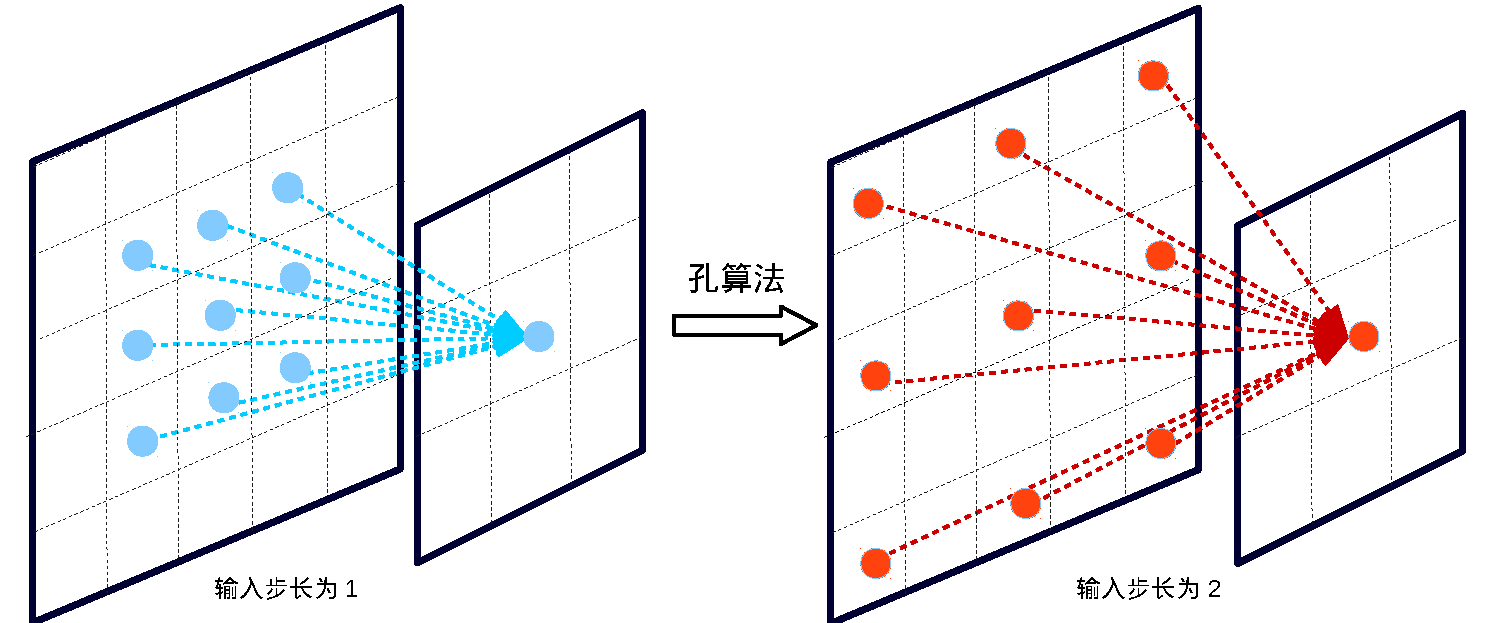
\includegraphics[width=0.618\textwidth]{../image/chap04/illustration/hole.pdf}
        \caption{单张图像}
        \label{fig:hole}
    \end{figure}

\end{frame}

\begin{frame}

    \begin{block}{要点一}
        \begin{itemize}
            \item 条目一
            \item 条目二
        \end{itemize}
    \end{block}

    \begin{figure} %文中的Grid-LSTM模型做的语义图像分割的例子
        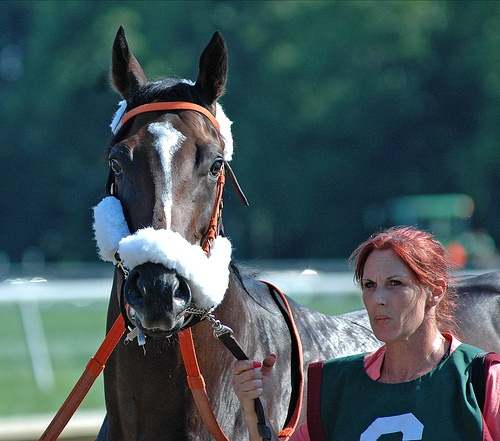
\includegraphics[width=.2\textwidth,height=.15\textwidth]{../image/chap04/example/2007_000799.jpg}
        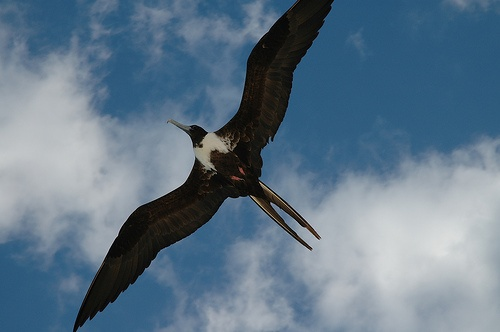
\includegraphics[width=.2\textwidth,height=.15\textwidth]{../image/chap04/example/2007_002094.jpg}
        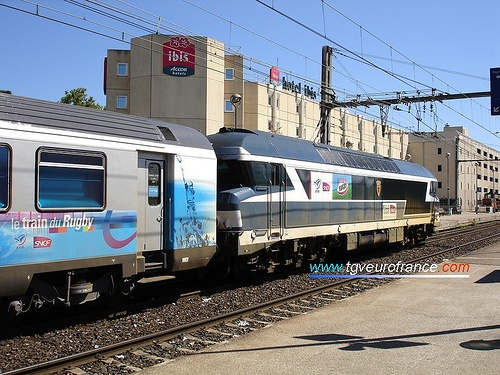
\includegraphics[width=.2\textwidth,height=.15\textwidth]{../image/chap04/example/2007_004483.jpg}
        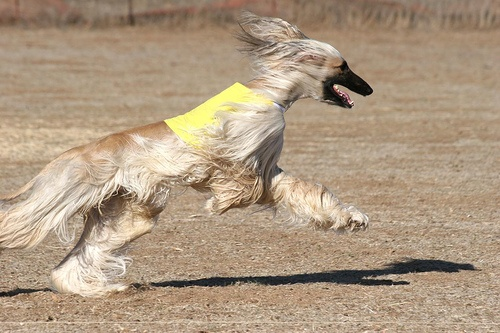
\includegraphics[width=.2\textwidth,height=.15\textwidth]{../image/chap04/example/2007_003194.jpg}
        \\
        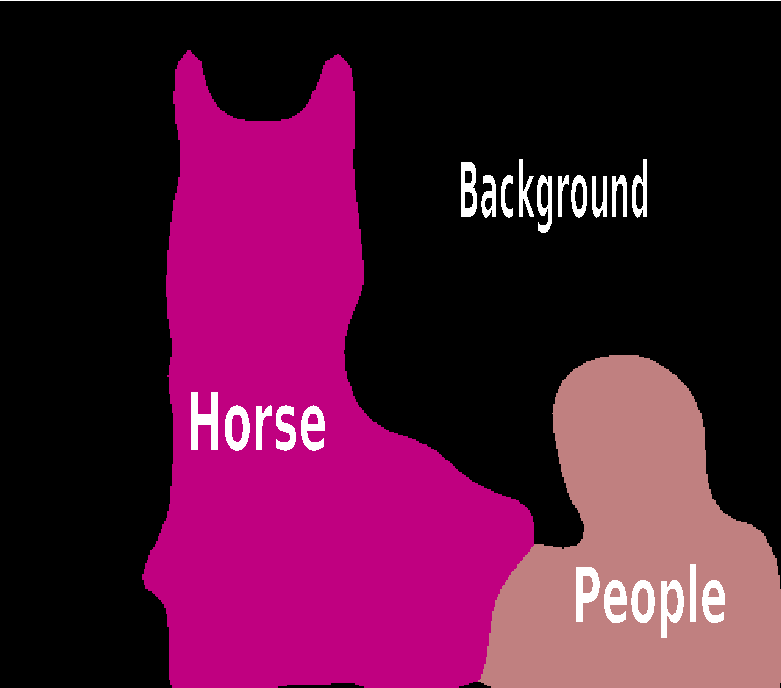
\includegraphics[width=.2\textwidth,height=.15\textwidth]{../image/chap04/example/2007_000799.pdf}
        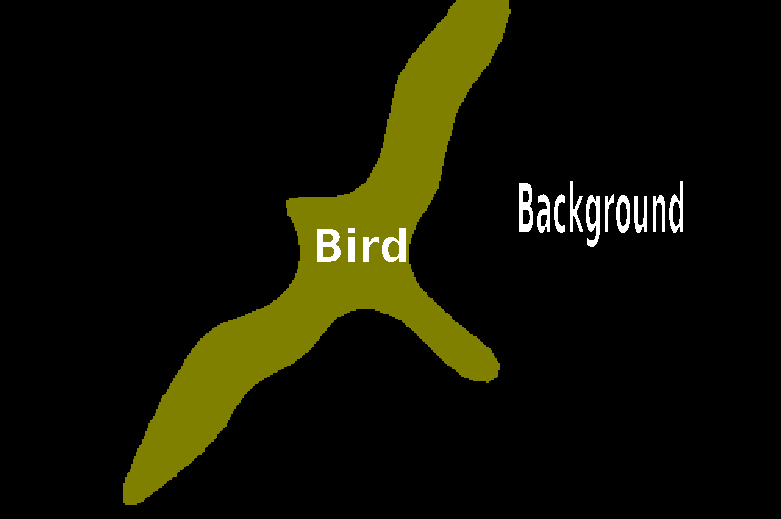
\includegraphics[width=.2\textwidth,height=.15\textwidth]{../image/chap04/example/2007_002094.pdf}
        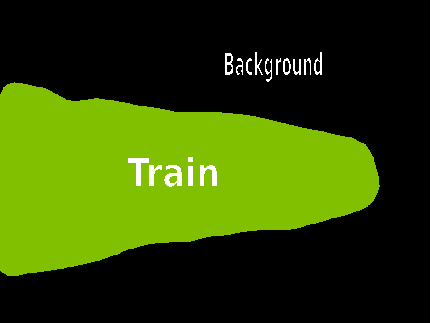
\includegraphics[width=.2\textwidth,height=.15\textwidth]{../image/chap04/example/2007_004483.pdf}
        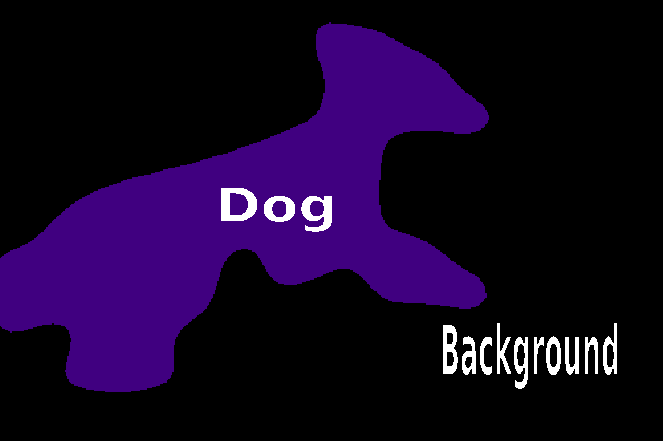
\includegraphics[width=.2\textwidth,height=.15\textwidth]{../image/chap04/example/2007_003194.pdf}
        \caption{并排的多张图像}
        \label{fig:multi-image-example1}
    \end{figure}

\end{frame}

\subsection{单页双图}

\begin{frame}

    \begin{block}{要点一}
        \begin{itemize}
            \item 条目一
            \item 条目二
        \end{itemize}
    \end{block}

    \begin{figure}
        \begin{minipage}{0.49\textwidth}
            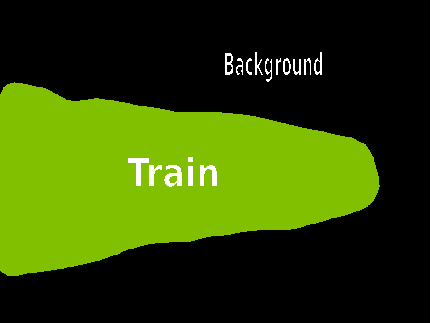
\includegraphics[height=0.45\textheight]{../image/chap04/example/2007_004483.pdf}
            \caption{一}
        \end{minipage}
        \begin{minipage}{0.49\textwidth}
            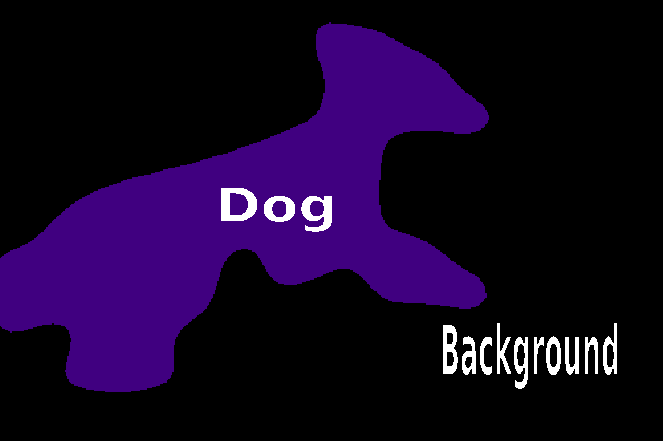
\includegraphics[height=0.45\textheight]{../image/chap04/example/2007_003194.pdf}
            \caption{二}
        \end{minipage}
    \end{figure}

\end{frame}

\subsection{单页大图}

\begin{frame}

    \begin{figure}
        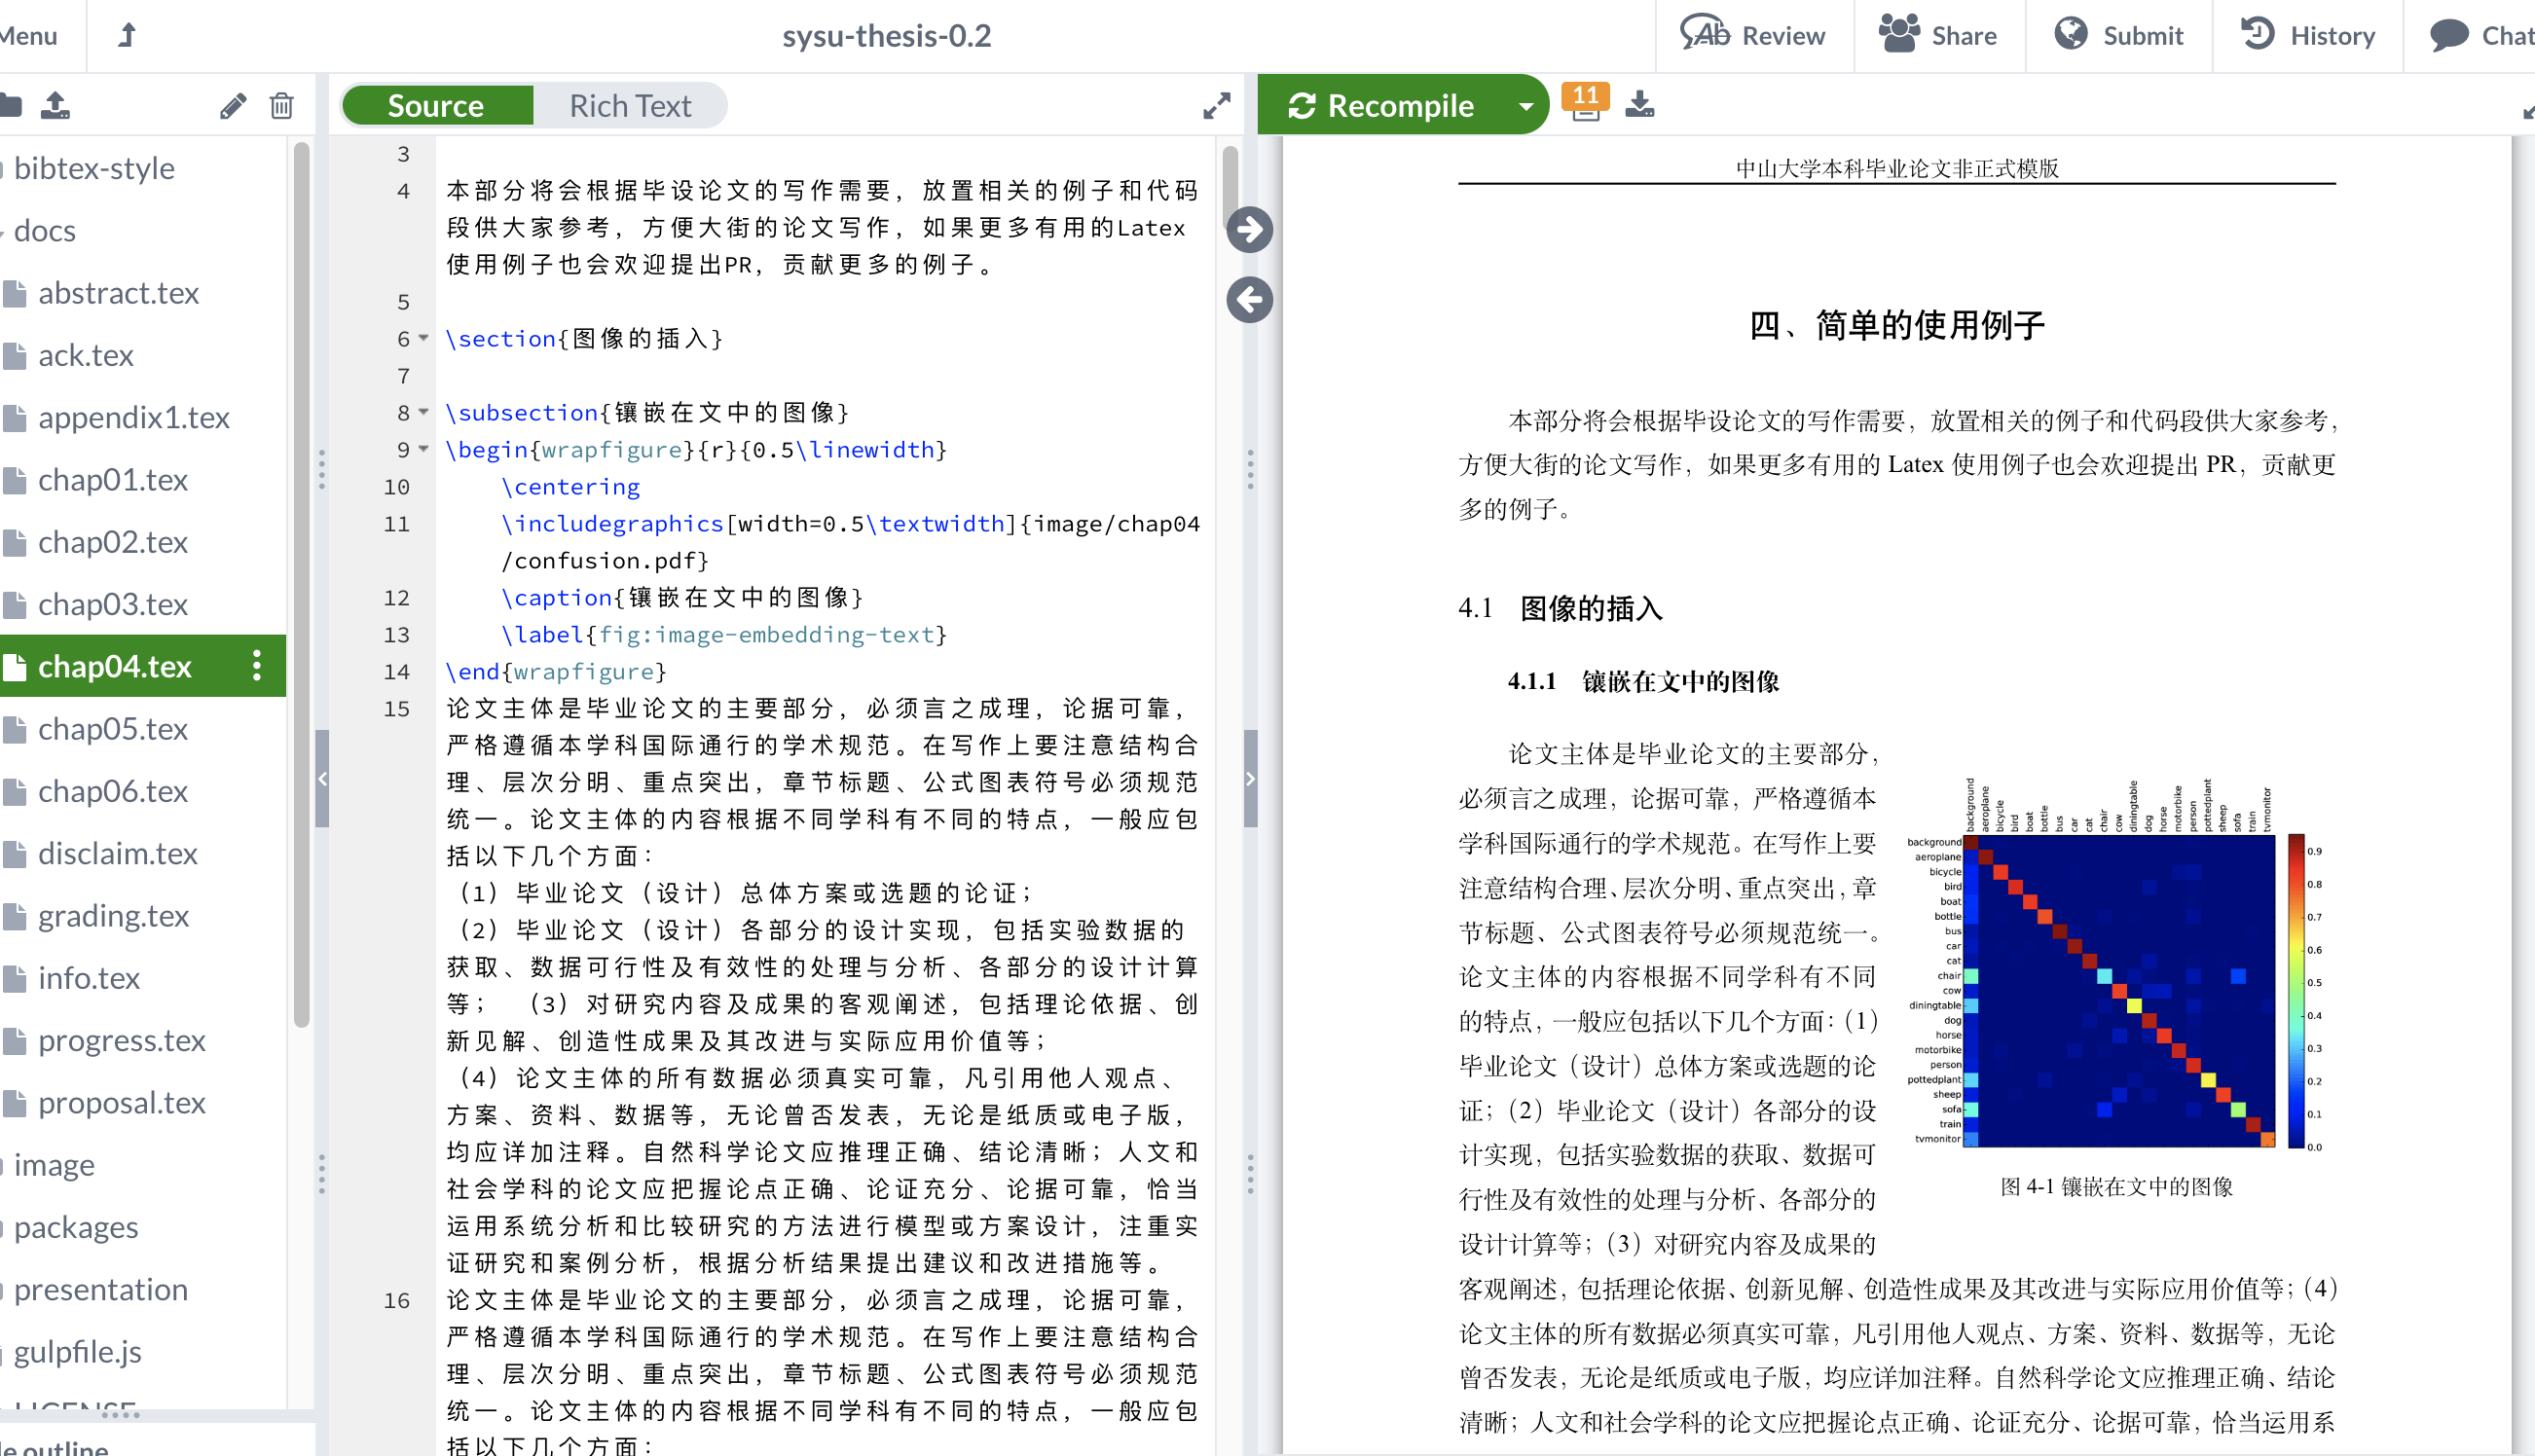
\includegraphics[width=0.9\textwidth]{../image/chap03/overleaf-example.jpg}
        \caption{Overleaf使用例子,这里的描述可以长一些}
        \label{fig:overleaf-example}
    \end{figure}

\end{frame}

\section{算法设计}

\subsection{图像搭配单页说明}

\begin{frame}

    \begin{block}{再试试公式}
        \begin{itemize}
            \item 看下面!
        \end{itemize}
    \end{block}

    \begin{equation}
        e^{i\pi}+1=0
    \end{equation}

\end{frame}

\section{实验与结果}

\begin{frame}

    \begin{block}{最后还有表格}
        \begin{itemize}
            \item 往下看!
        \end{itemize}
    \end{block}

    \begin{table}
        \begin{tabular}{ccc}
            \hline
            姓名       & 学号 & 性别   \\
            \hline
            Steve Jobs & 001  & Male   \\
            Bill Gates & 002  & Female \\
            \hline
        \end{tabular}
        \caption{表格示例,乱写的}
        \label{fig:table-example}
    \end{table}

\end{frame}

\section{总结与展望}

\subsection{其他块语法示例}

\begin{frame}

    \begin{block}{带标号的条目\footnote{引用一}}
        \begin{enumerate}
            \item 条目一,每一行字不要太密
            \item 条目二
        \end{enumerate}
    \end{block}

    \begin{alertblock}{重要理论}
        \begin{itemize}
            \item 条目一\footnote{引用二}和\alert{高亮字色}
        \end{itemize}
    \end{alertblock}

    \begin{examples}
        \begin{itemize}
            \item 举个栗子
        \end{itemize}
    \end{examples}

\end{frame}

\section{Q \& A}

\begin{frame}

    \begin{block}{Questions?}
        ~\\
        ~\\
        \center{\Large{Thank you!}}\\
        ~\\
        ~\\
        ~\\
        ~\\
    \end{block}

\end{frame}
\end{document}